\section{The estimate about box office influences of actors and directors}
\label{sec:impact}
\par The goal of this module is to find who is the most bankable person in a movie and to capture the dynamic trends about actors and directors during the period of a movie released. As figure \ref{fig:influ} shows, the box office influences can be made up of three parts: the actors'/directs' own box office appeal, media exposure and feedback from audience. For simplify, we regard actors and directors as creators.

\subsection{Contribution of Creators}
\begin{figure}[!htbp]
\centering
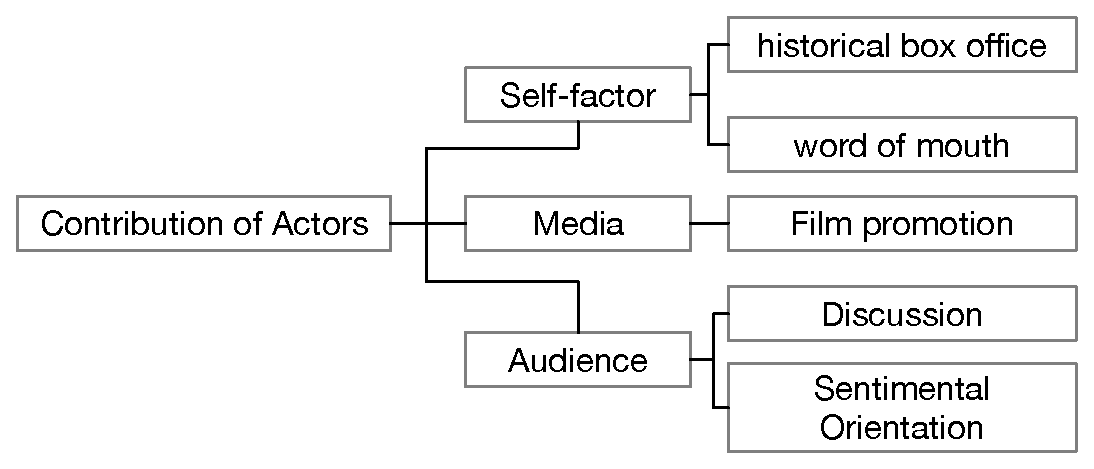
\includegraphics[width=0.8\columnwidth]{impact.eps}
\caption{Composition of creative influence}
\label{fig:influ}
\end{figure}
\par The creator's own box office appeal. Actor's own box office appeal includes historical box office results and historical word of mouth performance, in which the film's historical movie box office performance can objectively reflect the creative ability of gold absorption, while the historical reputation score can objectively reflect the creative performance by Audience recognition, so this article at the same time using the history of the box office and the history of reputation to measure the creative box office call ability.\\
\par We define the box office quality $boq$ to measure the box office generated by the creator itself based on the historical film data. 
As for directors, we define $boq(c)=wms(c)\cdot bos(c)$.Considering different role importance, as for actors, we define $boq(c) = f(c)\cdot wms(c)\cdot bos(c)$, where $f(c)$ is the influence factor and it depends on the position $k$ that the actor $c$ is. The larger $k$ is , the smaller $f(c)$ gets.\\
\par Media exposure. The movie's promotional period is always accompanied by a wide range of media coverage, the media's title content reflects the current public focus, if an actor or director appear in the title a lot, you can explain the public familiarity and attention more. We define $meq_j(c)$ as the number of times the creator $c$ referred to by the media in the $j$th week.\\
\par Feedback from the audience. Liu \cite{liu2006word} mentioned the impact of word-of-mouth on the box office is very large and Craig \cite{craig2015word}added to the equation online buzz variables expressing awareness and purchase intention and examined factors that contributed to higher levels of e-WOM. With the rapid development of the Internet, people can express their emotions on social media at any time. Thanks to the development of social media networks, the promotion of the movie has also gradually increased the proportion of online publicity. At the same time, the content of the discussion of the movie has also formed a considerable amount of data. The movie review often includes the concept of " If you can get the audience's idea of ​​an actor or master from the commentary, you can see whether the source of the audience's emotional inclination toward the movie comes from the influence of the movie's main actor (including the protagonist).We define $aco_j(c)$ as the number of times the creator $c$ referred to by the active comments in the $j$th week.\\\\
\subsection{Dynamic Impact of Creators}
\par In the short life of the movie, the contribution of the genre to the box office is obviously not constant. With the development of the Internet media, real-time feedback of the movie users on the movie will affect the watching desire of the non-movie users, and the positive contribution Refers to the potential box office or the desire to watch the increase; the negative is the box office to bring the negative image, to dispel the wishes of watching. Therefore, in the film's life, the star effect on the box office's contribution is dynamic, the project will be divided into the life of the movie before the release, the first week of release, the second week of release, the third week of release, released the fourth Friday A period, respectively, to explore the five periods of major box office contributions. \\
\par We define the DIR (Dynamic Impact Ratio) as $DIR_j(c)=\frac{DIP_j(c)}{\sum_{k\in C}DIP_j(k)}$ to measure the ratio of the box office contribute from creator $c$ to all box box office contribute in $j$th week, where 
\begin{equation}
DIP_j(c)=w_1\frac{boq(c)}{\sum_{c}boq(c)}+w_2\frac{\sum_{i=0}^{j}mep_j(c)}{\sum_{i=0}^{j}\sum_{c}mep_j(c)}+w_3\frac{\sum_{i=0}^{j}aco_i(c)}{\sum_{i=0}^{j}\sum_{c}aco_i(c)}
\end{equation}
where $w_1$,$w_2$,$w_3$ is three coefficients to embody the importance of creator's own box-office appleal, media exposure and feedback from the audience. In practice, we set $w_1=0.1,w_2=0.2,w_3=0.7$.

\begin{figure}[!htbp]
\centering
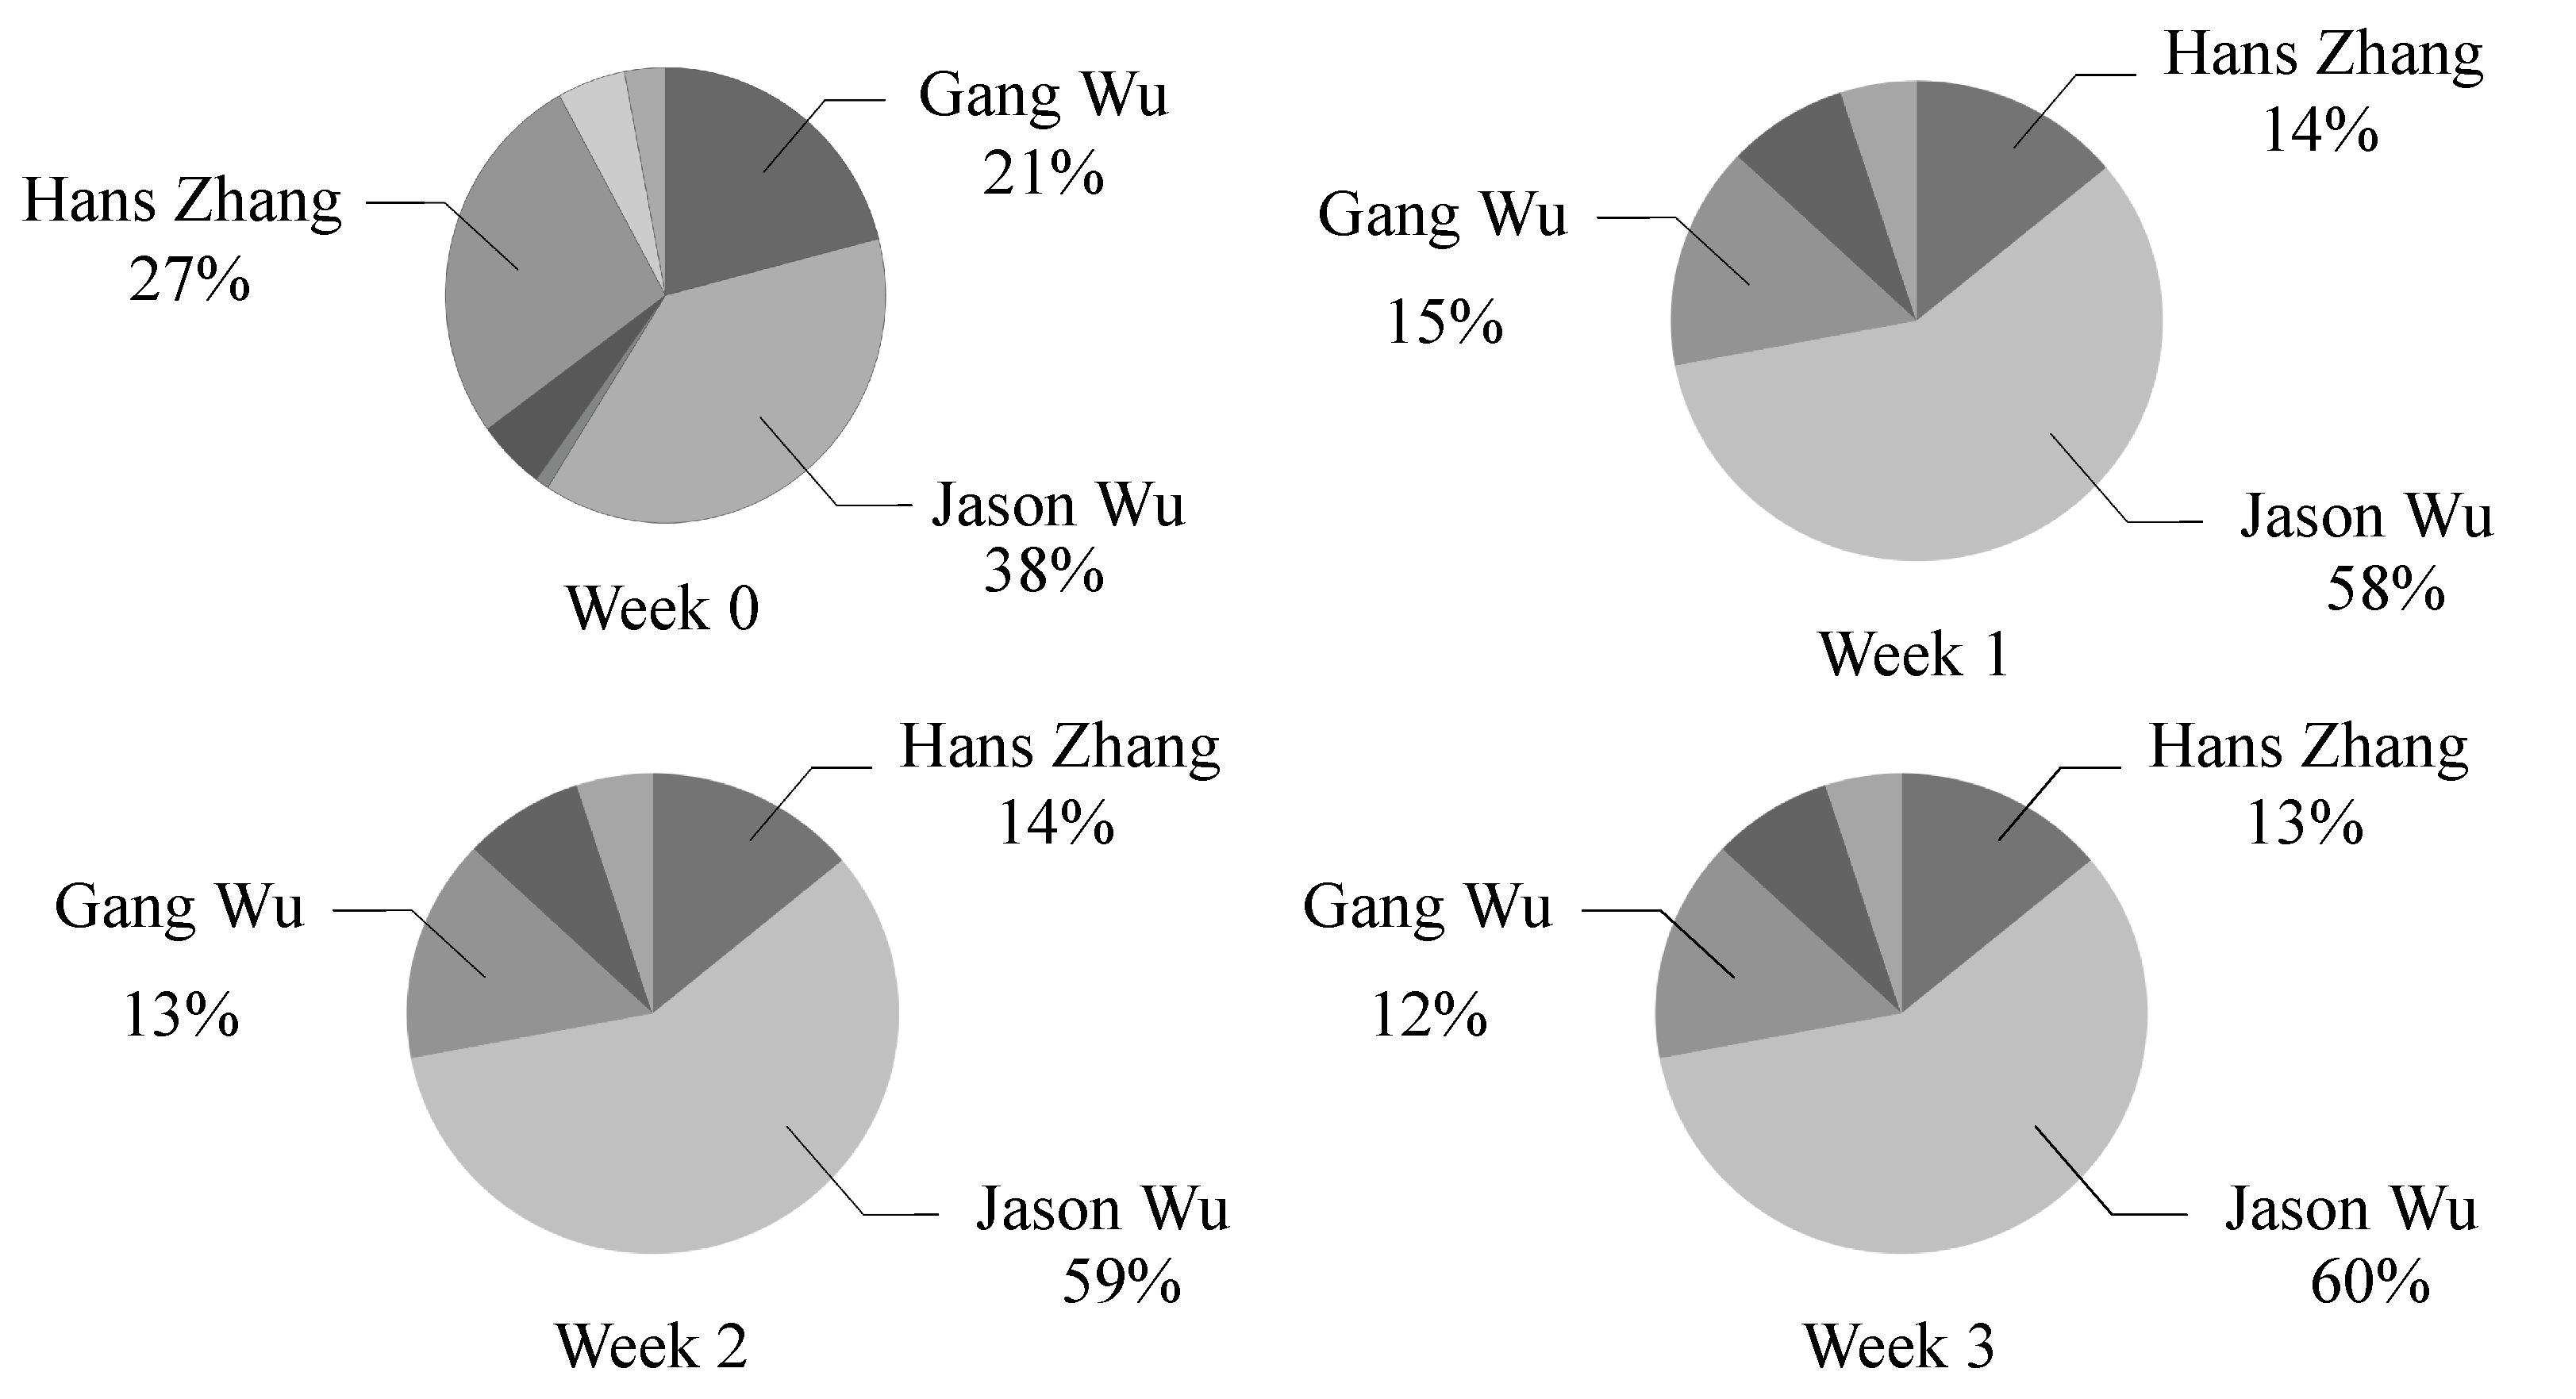
\includegraphics[width=0.8\columnwidth]{dynamicimpact.eps}
\caption{Changes of Wolf Warriors II}
\label{fig:ww}
\end{figure}

\par Figure \ref{fig:ww} shows dynamic impact of creators in "Wolf Warriors II". Before the movie released (week 0), the attentions people payed to Hans Zhang, Gang Wu and Jason Wu were equal while with the movie's release and the increase in the heat of the film, more and more people went to the movies for the sake of Jason Wu. Meanwhile, the dynamic influence process can reflect a major change in the importance of the movie. We can see that Jason Wu has greatly improved his value through the movie himself.